
\documentclass[letterpaper,hide notes,xcolor={table,svgnames},pdftex,10pt]{beamer}
\def\showexamples{t}

\usecolortheme{crane}
\setbeamertemplate{navigation symbols}{}

\usetheme{MyPittsburgh}
\usepackage{hyperref}
\usepackage{graphicx,xspace}
\usepackage[normalem]{ulem}
\usepackage{multicol}
\usepackage{amsmath,amssymb,amsthm,graphicx,xspace}
\newcommand\SF[1]{$\bigstar$\footnote{SF: #1}}

\usepackage[sfdefault,lf]{carlito}
\usepackage[T1]{fontenc}
\usepackage[scaled]{beramono}
\usepackage{tikzpagenodes}
\newcommand{\Rplus}{\protect\hspace{-.1em}\protect\raisebox{.35ex}{\small{\small\textbf{+}}}}
\newcommand{\Cpp}{\mbox{C\Rplus\Rplus}\xspace}

\newcounter{tmpnumSlide}
\newcounter{tmpnumNote}

\newcommand\mnote[1]{%
	\addtocounter{tmpnumSlide}{1}
	\ifdefined\showcues {~\tiny\fbox{\arabic{tmpnumSlide}}}\fi
	\note{\setlength{\parskip}{1ex}\addtocounter{tmpnumNote}{1}\textbf{\Large \arabic{tmpnumNote}:} {#1\par}}}

\newcommand\mmnote[1]{\note{\setlength{\parskip}{1ex}#1\par}}


\newcommand\mquestion[2]{{~\color{red}\fbox{?}}\note{\setlength{\parskip}{1ex}\par{\Large \textbf{?}} #1} \note{\setlength{\parskip}{1ex}\par{\Large \textbf{A}} #2\par}\ifdefined \presentationonly \pause \fi}

\newcommand\blackboard[1]{%
	\ifdefined   \showblackboard
		{#1}
	\else {\begin{center} \fbox{\colorbox{blue!30}{%
						\begin{minipage}{.95\linewidth}%
							\hspace{\stretch{1}} Some space intentionally left blank; done at the blackboard.%
						\end{minipage}}}\end{center}}%
	\fi%
}

\usepackage{listings}
\lstset{%
	keywordstyle=\bfseries,
	aboveskip=15pt,
	belowskip=15pt,
	captionpos=b,
	identifierstyle=\ttfamily,
	frame=lines,
	numbers=left, basicstyle=\scriptsize, numberstyle=\tiny, stepnumber=0, numbersep=2pt}

\usepackage{siunitx}
\newcommand\sius[1]{\num[group-separator = {,}]{#1}\si{\micro\second}}
\newcommand\sims[1]{\num[group-separator = {,}]{#1}\si{\milli\second}}
\newcommand\sins[1]{\num[group-separator = {,}]{#1}\si{\nano\second}}
\sisetup{group-separator = {,}, group-digits = true}

%% -------------------- tikz --------------------
\usepackage{tikz}
\usetikzlibrary{positioning}
\usetikzlibrary{arrows,backgrounds,automata,decorations.shapes,decorations.pathmorphing,decorations.markings,decorations.text}

\tikzstyle{place}=[circle,draw=blue!50,fill=blue!20,thick, inner sep=0pt,minimum size=6mm]
\tikzstyle{transition}=[rectangle,draw=black!50,fill=black!20,thick, inner sep=0pt,minimum size=4mm]

\tikzstyle{block}=[rectangle,draw=black, thick, inner sep=5pt]
\tikzstyle{bullet}=[circle,draw=black, fill=black, thin, inner sep=2pt]

\tikzstyle{pre}=[<-,shorten <=1pt,>=stealth',semithick]
\tikzstyle{post}=[->,shorten >=1pt,>=stealth',semithick]
\tikzstyle{bi}=[<->,shorten >=1pt,shorten <=1pt, >=stealth',semithick]

\tikzstyle{mut}=[-,>=stealth',semithick]

\tikzstyle{treereset}=[dashed,->, shorten >=1pt,>=stealth',thin]

\usepackage{ifmtarg}
\usepackage{xifthen}
\makeatletter
% new counter to now which frame it is within the sequence
\newcounter{multiframecounter}
% initialize buffer for previously used frame title
\gdef\lastframetitle{\textit{undefined}}
% new environment for a multi-frame
\newenvironment{multiframe}[1][]{%
	\ifthenelse{\isempty{#1}}{%
		% if no frame title was set via optional parameter,
		% only increase sequence counter by 1
		\addtocounter{multiframecounter}{1}%
	}{%
		% new frame title has been provided, thus
		% reset sequence counter to 1 and buffer frame title for later use
		\setcounter{multiframecounter}{1}%
		\gdef\lastframetitle{#1}%
	}%
	% start conventional frame environment and
	% automatically set frame title followed by sequence counter
	\begin{frame}%
		\frametitle{\lastframetitle~{\normalfont(\arabic{multiframecounter})}}%
		}{%
	\end{frame}%
}
\makeatother

\makeatletter
\newdimen\tu@tmpa%
\newdimen\ydiffl%
\newdimen\xdiffl%
\newcommand\ydiff[2]{%
	\coordinate (tmpnamea) at (#1);%
	\coordinate (tmpnameb) at (#2);%
	\pgfextracty{\tu@tmpa}{\pgfpointanchor{tmpnamea}{center}}%
	\pgfextracty{\ydiffl}{\pgfpointanchor{tmpnameb}{center}}%
	\advance\ydiffl by -\tu@tmpa%
}
\newcommand\xdiff[2]{%
	\coordinate (tmpnamea) at (#1);%
	\coordinate (tmpnameb) at (#2);%
	\pgfextractx{\tu@tmpa}{\pgfpointanchor{tmpnamea}{center}}%
	\pgfextractx{\xdiffl}{\pgfpointanchor{tmpnameb}{center}}%
	\advance\xdiffl by -\tu@tmpa%
}
\makeatother
\newcommand{\copyrightbox}[3][r]{%
	\begin{tikzpicture}%
		\node[inner sep=0pt,minimum size=2em](ciimage){#2};
		\usefont{OT1}{phv}{n}{n}\fontsize{4}{4}\selectfont
		\ydiff{ciimage.south}{ciimage.north}
		\xdiff{ciimage.west}{ciimage.east}
		\ifthenelse{\equal{#1}{r}}{%
			\node[inner sep=0pt,right=1ex of ciimage.south east,anchor=north west,rotate=90]%
			{\raggedleft\color{black!50}\parbox{\the\ydiffl}{\raggedright{}#3}};%
		}{%
			\ifthenelse{\equal{#1}{l}}{%
				\node[inner sep=0pt,right=1ex of ciimage.south west,anchor=south west,rotate=90]%
				{\raggedleft\color{black!50}\parbox{\the\ydiffl}{\raggedright{}#3}};%
			}{%
				\node[inner sep=0pt,below=1ex of ciimage.south west,anchor=north west]%
				{\raggedleft\color{black!50}\parbox{\the\xdiffl}{\raggedright{}#3}};%
			}
		}
	\end{tikzpicture}
}


%% --------------------

%\usepackage[excludeor]{everyhook}
%\PushPreHook{par}{\setbox0=\lastbox\llap{MUH}}\box0}

%\vspace*{\stretch{1}

%\setbox0=\lastbox \llap{\textbullet\enskip}\box0}

\setlength{\parskip}{\fill}

\newcommand\noskips{\setlength{\parskip}{1ex}}
\newcommand\doskips{\setlength{\parskip}{\fill}}

\newcommand\xx{\par\vspace*{\stretch{1}}\par}
\newcommand\xxs{\par\vspace*{2ex}\par}
\newcommand\tuple[1]{\langle #1 \rangle}
\newcommand\code[1]{{\sf \footnotesize #1}}
\newcommand\ex[1]{\uline{Example:} \ifdefined \presentationonly \pause \fi
	\ifdefined\showexamples#1\xspace\else{\uline{\hspace*{2cm}}}\fi}

\newcommand\ceil[1]{\lceil #1 \rceil}


\AtBeginSection[]
{
	\begin{frame}
		\frametitle{Outline}
		\tableofcontents[currentsection]
	\end{frame}
}



\pgfdeclarelayer{edgelayer}
\pgfdeclarelayer{nodelayer}
\pgfsetlayers{edgelayer,nodelayer,main}

\tikzstyle{none}=[inner sep=0pt]
\tikzstyle{rn}=[circle,fill=Red,draw=Black,line width=0.8 pt]
\tikzstyle{gn}=[circle,fill=Lime,draw=Black,line width=0.8 pt]
\tikzstyle{yn}=[circle,fill=Yellow,draw=Black,line width=0.8 pt]
\tikzstyle{empty}=[circle,fill=White,draw=Black]
\tikzstyle{bw} = [rectangle, draw, fill=blue!20,
text width=4em, text centered, rounded corners, minimum height=2em]

\newcommand{\CcNote}[1]{% longname
	This work is licensed under the \textit{Creative Commons #1 3.0 License}.%
}
\newcommand{\CcImageBy}[1]{%
	\includegraphics[scale=#1]{creative_commons/cc_by_30.pdf}%
}
\newcommand{\CcImageSa}[1]{%
	\includegraphics[scale=#1]{creative_commons/cc_sa_30.pdf}%
}
\newcommand{\CcImageNc}[1]{%
	\includegraphics[scale=#1]{creative_commons/cc_nc_30.pdf}%
}
\newcommand{\CcGroupBySa}[2]{% zoom, gap
	\CcImageBy{#1}\hspace*{#2}\CcImageNc{#1}\hspace*{#2}\CcImageSa{#1}%
}
\newcommand{\CcLongnameByNcSa}{Attribution-NonCommercial-ShareAlike}

\newenvironment{changemargin}[1]{% 
	\begin{list}{}{% 
		\setlength{\topsep}{0pt}% 
		\setlength{\leftmargin}{#1}% 
		\setlength{\rightmargin}{1em}
		\setlength{\listparindent}{\parindent}% 
		\setlength{\itemindent}{\parindent}% 
		      \setlength{\parsep}{\parskip}% 
		      }% 
		\item[]}{\end{list}}




\title{Lecture 22 --- Advanced Concurrency Problems }

\author{Jeff Zarnett \\ \small \texttt{jzarnett@uwaterloo.ca}}
\institute{Department of Electrical and Computer Engineering \\
	University of Waterloo}
\date{\today}


\begin{document}

\begin{frame}
	\titlepage

\end{frame}


\begin{frame}
	\frametitle{Get A Pizza This!}
	\begin{center}
		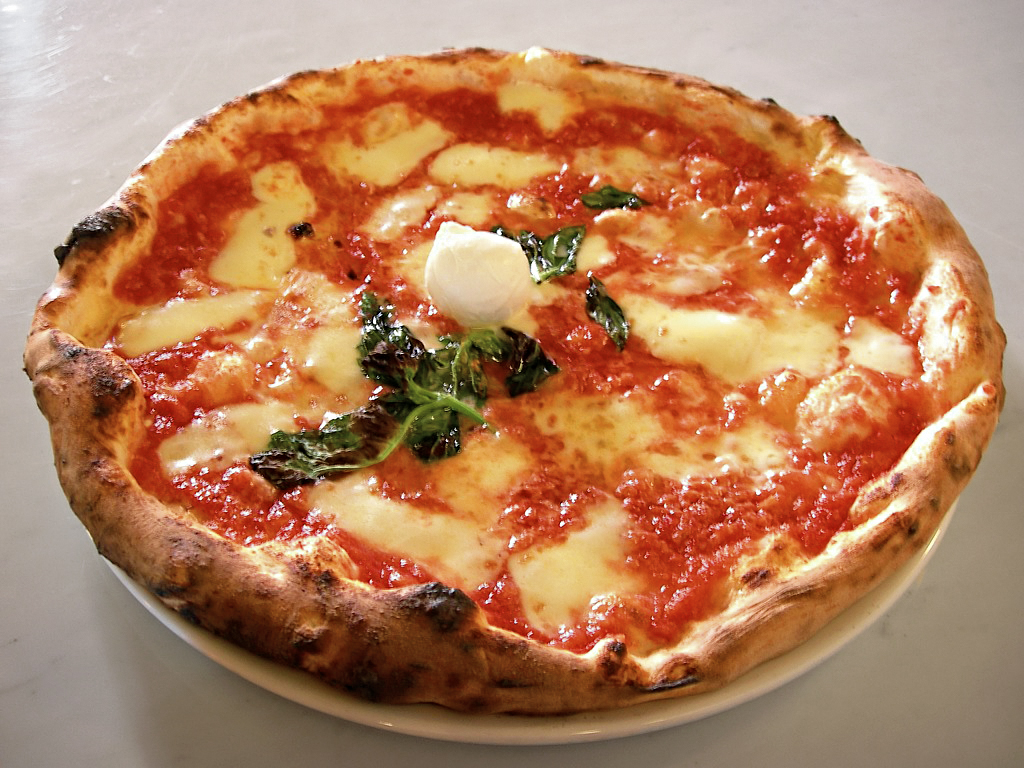
\includegraphics[width=0.7\textwidth]{images/pizza.jpg}
	\end{center}
	\hfill Image Credit: Valerio Capello

\end{frame}

\begin{frame}
	\frametitle{The Pizza Makers Problem}

	Let's consider a more advanced concurrency problem.

	It's also called the ``Cigarette Smokers Problem''.

	But smoking is bad for you.

	Pizza, while not exactly health food, is amazing. Delicious, delicious pizza.


\end{frame}


\begin{frame}
	\frametitle{Iron Chef: Pizza}
	\begin{center}
		
\includegraphics[width=0.5\textwidth]{images/ironchef.jpg}
	\end{center}

	A new show to be hosted by some famous TV chef personality is being pitched, and you're going to write a simulation of it.

	A pizza requires three ingredients: dough, sauce, and cheese.

\end{frame}

\begin{frame}
	\frametitle{This Could Be a Real Show}

	Each contestant has an unlimited supply of one ingredient.

	Contestant A has an unlimited supply of dough, Contestant B has an unlimited supply of sauce, and Contestant C has an unlimited supply of cheese.

	Each contestant needs to get the two ingredients they do not have and then can make a pizza.

	They will continue to (try to) make pizza in a loop until time is up.

\end{frame}

\begin{frame}
	\frametitle{Start the Show!}
	At the beginning of the episode, the host places two different random ingredients out.

	Contestants can signal the host to ask for more ingredients, but they should not do so unless they actually need some.

	Each time the host is woken up (signalled), he again places two different random ingredients out.

	When an ingredient is placed on the table, the host posts on the associated semaphore.

\end{frame}

\begin{frame}
	\frametitle{Is this Relevant?}

	In this scenario, there are resources provided by some external system and the contestants are processes that want resources.

	But we shouldn't be wasteful: resources should only be requested when they are needed and processes should take only what they need.

	Applications should only wake up if they can do something useful.

\end{frame}

\begin{frame}
	\frametitle{How Hard Do You Want It To Be?}

	There are some restrictions, though, and they could make the problem either impossible or trivial.

	In the impossible version, you can't modify what the host does (which is sensible, because you don't control the other system).

	But you also cannot use conditional (if) statements, which is pretty ridiculous.

\end{frame}

\begin{frame}
	\frametitle{All Too Easy}

	In the trivial version, the host tells which contestants whose turn it is.

	It requires the host system to know too much about the contestants.

	The interesting version has just the restriction that we can't control the host behaviour.



	\begin{center}
		
\includegraphics[width=0.5\textwidth]{images/fieri.jpg}
	\end{center}

	And he is a TV chef personality, after all, they do wacky things.


\end{frame}


\begin{frame}[fragile]
	\frametitle{Let's Make Some Pizza!}
	All semaphores start at 0, except for \texttt{host} which starts as 1 (so the host will run the first time). Does this work?

	\begin{multicols}{3}
		\textbf{Contestant A}
		\begin{lstlisting}
wait( sauce )
get_sauce()
wait( cheese )
get_cheese()
make_pizza( )
post( host )
\end{lstlisting}
		\columnbreak
		\textbf{Contestant B}
		\begin{lstlisting}
wait( dough )
get_dough()
wait( cheese )
get_cheese()
make_pizza( )
post( host )
\end{lstlisting}
		\columnbreak
		\textbf{Contestant C}
		\begin{lstlisting}
wait( sauce )
get_sauce()
wait( dough )
get_dough()
make_pizza( )
post( host )
\end{lstlisting}
	\end{multicols}

\end{frame}


\begin{frame}
	\frametitle{Him Again!}

	No. Deadlock can easily occur.

	Suppose the host puts out sauce and dough.

	If contestant B takes the dough and contestant A takes the sauce, then both of them are blocked and nobody can proceed and nobody gets pizza.

\end{frame}


\begin{frame}
	\frametitle{This Isn't What I Ordered...}

	Part of the problem here is that a contestant doesn't have a good way to assess what the ingredients are before going up there.

	And once there, if it finds that the ingredients match someone else's needs, we don't call that contestant over.

	That would be clever, but to make this work we would need a way to ``check'' what ingredients are there and semaphores don't let us do that.

	Can we work with what we have?

\end{frame}

\begin{frame}
	\frametitle{We Need a Sidekick!}
	\begin{center}
		
\includegraphics[width=0.4\textwidth]{images/robin.jpg}
	\end{center}

	Imagine now that each contestant gets a helper.

	The job of the helper is to, well, help their contestant to make pizza by figuring out whose turn it is.

\end{frame}


\begin{frame}
	\frametitle{Boolean Variables}

	For this there are boolean variables \texttt{dough\_present}, \texttt{sauce\_present}, and \texttt{cheese\_present}

	They are all initialized to \texttt{false}.

	They are protected by a semaphore (called \texttt{mutex}).

	The helpers update that variable, and based on the information available, signal which contestant should come up to the table and take ingredients.

\end{frame}

\begin{frame}[fragile]
	\frametitle{Working with a Sidekick}

	Each contestant now has a semaphore (such as \texttt{contestantA} for contestant A) which the helpers will post on.

	Contestants are still responsible for telling the host to put out more ingredients.

	\begin{multicols}{3}
		\textbf{Helper 1}
		\begin{lstlisting}
wait( sauce )
wait( mutex )
if dough_present  
  dough_present = false;
  post( contestantC )
else if cheese_present
  cheese_present = false;
  post( contestantA )
else
  sauce_present = true;
end if  
post( mutex )
\end{lstlisting}
		\columnbreak
		\textbf{Helper 2}
		\begin{lstlisting}
wait( dough )
wait( mutex )
if sauce_present  
  sauce_present = false;
  post( contestantC )
else if cheese_present
  cheese_present = false;
  post( contestantB )
else
  dough_present = true;
end if  
post( mutex )
\end{lstlisting}
		\columnbreak
		\textbf{Helper 3}
		\begin{lstlisting}
wait( cheese )
wait( mutex )
if dough_present  
  dough_present = false;
  post( contestantB )
else if sauce_present
  sauce_present = false;
  post( contestantA )
else
  cheese_present = true;
end if  
post( mutex )
\end{lstlisting}
	\end{multicols}

\end{frame}

\begin{frame}
	\frametitle{Analyzing the Helper}

	So let's analyze Helper 1.

	In this case, the helper is woken up when sauce is placed on the table.

	It then locks the mutex so that it can manipulate the shared variables of what ingredients are present.

	Now we decide what to do here.

	Obviously, each of the other helpers will signal the appropriate contestant based on its assessment of the state of the ingredients.

\end{frame}


\begin{frame}[fragile]
	\frametitle{Working with a Sidekick}

	\begin{multicols}{3}
		\textbf{Contestant A}
		\begin{lstlisting}
wait( contestantA )
get_sauce()
get_cheese()
make_pizza( )
post( host )
\end{lstlisting}
		\columnbreak
		\textbf{Contestant B}
		\begin{lstlisting}
wait( contestantB )
get_dough()
get_cheese()
make_pizza( )
post( host )
\end{lstlisting}
		\columnbreak
		\textbf{Contestant C}
		\begin{lstlisting}
wait( contestantC )
get_sauce()
get_dough()
make_pizza( )
post( host )
\end{lstlisting}
	\end{multicols}

	The contestant code is pretty much trivial now: wait until a helper signals, then go take your ingredients and make a pizza.

	Once the pizza is in the oven, indicate that you are ready for more ingredients.

\end{frame}

\begin{frame}
	\frametitle{Rule Change}

	The generalized version of the problem is what happens when the host puts out ingredients periodically, without a need to be signalled to ask for more.

	How do we modify the solution to deal with that?

	If there is no longer a need for the contestants to signal that they want more resources, \texttt{post( host )} in the contestant code has to be removed.

	But what about the helpers?

\end{frame}

\begin{frame}
	\frametitle{How Many Dough?}

	Instead of boolean variables to indicate the presence or absence of an ingredient what we need instead is an integer counter to know how many there are.

	They are: \texttt{num\_dough}, \texttt{num\_sauce}, and \texttt{num\_cheese}, and they all start as zero.

\end{frame}

\begin{frame}[fragile]
	\frametitle{Updated Sidekick Code}

	\begin{multicols}{3}
		\textbf{Helper 1}
		\begin{lstlisting}
wait( sauce )
wait( mutex )
if num_dough > 0  
  num_dough--
  post( contestantC )
else if num_cheese > 0
  num_cheese--
  post( contestantA )
else
  num_sauce++
end if  
post( mutex )
\end{lstlisting}
		\columnbreak
		\textbf{Helper 2}
		\begin{lstlisting}
wait( dough )
wait( mutex )
if num_sauce > 0  
  num_sauce--
  post( contestantC )
else if num_cheese > 0
  num_cheese--
  post( contestantB )
else
  num_dough++
end if  
post( mutex )
\end{lstlisting}
		\columnbreak
		\textbf{Helper 3}
		\begin{lstlisting}
wait( cheese )
wait( mutex )
if num_dough > 0 
  num_dough--
  post( contestantB )
else if num_sauce > 0
  num_sauce--
  post( contestantA )
else
  num_cheese++
end if  
post( mutex )
\end{lstlisting}
	\end{multicols}

	This pattern is referred to as the ``scoreboard''.

	As threads go about their actions, they take a look at the current state (the scoreboard) and decide how to act based on that.

\end{frame}

\begin{frame}
	\frametitle{Barber of Seville}

	\begin{center}
		
\includegraphics[width=0.7\textwidth]{images/rabbitofseville.jpg}
	\end{center}

\end{frame}

\begin{frame}
	\frametitle{The Barbershop Problem}

	Consider the ``Barbershop Problem'', originally proposed by Dijkstra.

	A barbershop is a place where customers get their hair cut.

	A barbershop consists of a waiting area with $n$ chairs, and a barber chair.

\end{frame}


\begin{frame}
	\frametitle{Barbershop Behaviour}

	If there are no customers to be served, the barber goes to sleep.

	If a customer enters the barbershop and all chairs are occupied, then the customer leaves the shop.

	If the barber is busy, but chairs are available, then the customer sits in one of the free chairs.

	If the barber is asleep, the customer wakes up the barber.

\end{frame}

\begin{frame}
	\frametitle{Wake Up!}

	Customer threads should call \texttt{get\_hair\_cut()} when it is their turn.

	If the shop is full, the customer should \texttt{return} (exit/leave).

	The barber thread will call \texttt{cut\_hair}.

	The barber can cut only one person's hair at a time, so there should be exactly one thread calling \texttt{get\_hair\_cut()} concurrently.

	You can assume that external forces cause customers to appear and the barber to keep working.

\end{frame}


\begin{frame}
	\frametitle{Scoreboard Pattern Again}


	We need an integer counter for customers waiting called \texttt{customers} that starts at 0.

	We will also have a mutex for controlling access to \texttt{customers} called \texttt{mutex} (it obviously starts at 1).

	Finally, two semaphores, \texttt{customer} and \texttt{barber} that both start at 0.

	Let's write down some outline of the barber and customer code...

\end{frame}


\begin{frame}[fragile]
	\frametitle{Barbershop Solution}

	\begin{multicols}{2}
		\textbf{Customer}
		\begin{lstlisting}
wait( mutex )
if customers == n
    signal( mutex )
    return
end if
customers++
signal( mutex )

signal( customer )
wait( barber )
get_hair_cut()

wait( mutex )
customers--
signal( mutex )
\end{lstlisting}
		\columnbreak
		\textbf{Barber}
		\begin{lstlisting}
wait( customer )
signal( barber )
cut_hair()
  \end{lstlisting}
	\end{multicols}

	Is there a risk of deadlock?

	Starvation?

\end{frame}


\begin{frame}
	\frametitle{I WANT TO SPEAK TO A MANAGER}
	
	\begin{center}
	
\includegraphics[width=0.4\textwidth]{images/manager.jpg}
	\end{center}

	We can maybe say that customers who give up in frustration are disappointed.

	Is that better than making them wait forever?

	This is actually a good lesson for services in general.

\end{frame}


\begin{frame}
	\frametitle{SCIENCE!!!}

	\begin{center}
		
\includegraphics[width=0.5\textwidth]{images/h2o2.jpg}
	\end{center}


\end{frame}

\begin{frame}
	\frametitle{Science!}

	There are two kinds of thread, \texttt{oxygen()} and \texttt{hydrogen()}.

	As you will recall from basic chemistry, water, H$_{2}$O, requires two hydrogen modules and one oxygen module.

	To assemble the desired molecule (water) a group rendezvous pattern is needed to make each thread wait until all ingredients are present in the correct amounts.

	As each thread passes the barrier, it should call the function \texttt{bond()} which makes the water.

	Our solution must function so that all threads for one molecule invoke \texttt{bond()} before any of the threads from the next molecule do.

\end{frame}


\begin{frame}
	\frametitle{Water is Life}

	In the example, we'll assume the \texttt{oxygen} and \texttt{hydrogen} threads are created and started correctly and in the correct proportions.

	The code for the creation of those two types of threads is not shown.

	The reusable two-phase barrier from earlier has also been converted into C code.

	The oxygen queue and hydrogen queue start as ``locked''.

\end{frame}

\begin{frame}[fragile]
	\frametitle{Water is Life}

	\begin{lstlisting}[language=C]
int oxygen;
int hydrogen;
pthread_mutex_t barrier_mutex;
sem_t turnstile;
int barrier_count;
int barrier_N;
sem_t bond;
sem_t oxygen_queue;
sem_t hydrogen_queue;
\end{lstlisting}
\end{frame}

\begin{frame}[fragile]
	\frametitle{Water is Life}

	\begin{lstlisting}[language=C]
void barrier_enter( ) {
  pthread_mutex_lock( &barrier_mutex );
  barrier_count++;
  if ( barrier_count == barrier_N ) {
    sem_post( &turnstile );
  }
  pthread_mutex_unlock( &barrier_mutex );
  sem_wait( &turnstile );
  sem_post( &turnstile );            
}

void barrier_exit( ) {
  pthread_mutex_lock( &barrier_mutex );
  barrier_count--;
  if ( barrier_count == 0 ) {
    sem_wait( &turnstile );
  }
  pthread_mutex_unlock( &barrier_mutex );
}
\end{lstlisting}

\end{frame}

\begin{frame}[fragile]
	\frametitle{Water is Life}

	\begin{lstlisting}[language=C]
void* oxygen( void* ignore ) {
  sem_wait( &bond );
  oxygen++;
  
  if( hydrogen >= 2 ){
    sem_post( &hydrogen_queue );
    sem_post( &hydrogen_queue );
    hydrogen -= 2;
    sem_post( &oxygen_queue );
    oxygen--;
  } else {
    sem_post( &bond );
  }
  
  sem_wait( &oxygen_queue );
  bond();

  barrier_enter();
  barrier_exit();

  sem_post( &bond );
  
  pthread_exit( NULL )
}
\end{lstlisting}
\end{frame}


\begin{frame}[fragile]
	\frametitle{Water is Life}
	\begin{lstlisting}[language=C]
void* hydrogen( void* ignore ) {
  sem_wait( &bond );
  hydrogen++;
  
  if( hydrogen >= 2 && oxygen >= 1 )
    sem_post( &hydrogen_queue );
    sem_post( &hydrogen_queue );
    hydrogen -= 2;
    sem_post( &oxygen_queue );
    oxygen--;
  } else {
    sem_post( &bond );
  }
  
  sem_wait( &hydrogen_queue );
  bond();
  
  barrier_enter();
  barrier_exit();
  
  pthread_exit( NULL )
}
\end{lstlisting}
\end{frame}


\begin{frame}
	\frametitle{Analyzing the Solution}


	It is a little strange that the hydrogen threads don't post on \texttt{bond}.

	Isn't this a problem?

\end{frame}


\begin{frame}
	\frametitle{Posting Bond?}

	It turns out no, because the oxygen threads post on it unconditionally.

	When a thread arrives but the water molecule cannot be formed, whether it is oxygen or hydrogen, a post on \texttt{bond} takes place.

	Whoever waited on \texttt{bond} does not matter, as long as one of the threads that went into the water molecule posts on it before leaving.

	As the chemical composition of water has one oxygen, the job is assigned to this molecule.

\end{frame}



\begin{frame}
	\frametitle{The World is Big}

	These are by no means all the concurrency problems in the world.

	But for now we will leave it here, before  we get into really obscure problems...

\end{frame}

\end{document}

